\chapter{Progetto e attività di stage}
\textit{Questa capitolo parla delle attività di stage andando a descrivere il progetto nei suoi stati di avanzamento, le scelte adottate e le motivazioni che mi hanno permesso di prendere decisioni.}

\section{Formazione}
All'inizio dello stage, la prima attività che ho dovuto svolgere, è stata quella di studio delle applicazioni adottate dall'azienda. In aggiunta ho appreso i formalismi, ossia codici e abbreviazioni adottate per la realizzazione dei campi dei database. 
Per la formazione sull'applicazione \inde\, ho seguito sei video-corsi della durata di una/due ore l'uno. Per velocizzare l'apprendimento dell'uso dell'applicazione, il mio tutor mi ha richiesto di realizzare le applicazioni presenti nei video.
Rispetto a quanto pianificato, l'apprendimento del programma è risultato più rapido della settimana preventivata e quindi, durante la stessa, ho potuto interfacciarmi con i Data Warehouse e lo studio di alcune Stored Procedures. 
Al termine della prima settimana ho iniziato lo studio dei documenti relativi al configuratore catalogo/prodotti.


\section{Progettazione}
La seconda settimana di stage, divisa in incontri con il cliente e lavoro presso la sede di Castelfranco, ho iniziato ad affrontare le dinamiche aziendali concentrandomi sulle attività di progetto.

\subsection{Database}
Il primo punto affrontato durante il periodo di stage è stato il database. In questa fase sono stato affiancato dal tutor aziendale. Il cliente ci ha dato piena facoltà di agire, permettendoci di scegliere tra due possibili soluzioni: riutilizzare tabelle presenti nel database o crearne nuove. 
Il cliente, che dispone di sei applicazioni ideate con InDe, nei mesi di stage ha richiesto di avviare nuovi progetti.
Dopo un'attenta discussione con il cliente la scelta più consona è risultata essere quella di creare tabelle nuove. I nuovi componenti dovrebbero essere in futuro integrati in altre applicazioni.\\
Per cercare di mantenere uniformità e coerenza con il resto del Data Warehouse, si è optato di non inserire vincoli di Foreign Key.
Questa opzione avrebbe permesso di ottenere query più rapide ma in seguito ad alcune osservazioni, è risultato superfluo vista la velocità dei server. 
Tuttavia, continuo a ritenere molto utile la creazione delle foreign key. In questa maniera anche se le tabelle iniziano ad avere una quantità di record sproporzionata la velocità resta soddisfacente e/o elevata. Inoltre, il problema dell'eventuale plugin dell'applicazione richiede comunque che si modifichi il codice nell'importazione della componente. 
Quest'ultima scelta ha come vantaggio di estendere i progetti in maniera più rapida.
Infine, per concludere il tema vincoli, gli unici adottati sono quelli di Primary Key.
\\

La prima tabella da cui ho iniziato la progettazione è stata quella degli articoli. Quest'ultima è già presente nel data warehouse e dispone di una vista. Partendo da questi due contenitori, si è realizzata una struttura che permetta prima di creare una lista prodotti. Se l'articolo esiste è possibile arricchire le sue informazioni.\\

Gli aspetti da tenere in considerazione sono:
\begin{itemize}
	\item ogni articolo ha delle immagini, video o dei file di vario genere;
	\item ogni articolo deve poter avere uno o più tag;
	\item ogni articolo deve avere delle informazioni di base e delle informazioni aggiuntive;
	\item ogni informazione aggiuntiva deve poter essere gestita (creata, modificata ed eliminata).
\end{itemize}
Queste informazioni sono state definite durante la prima riunione presso la sede del cliente.\\

\begin{figure}[!h] 
	\centering 
	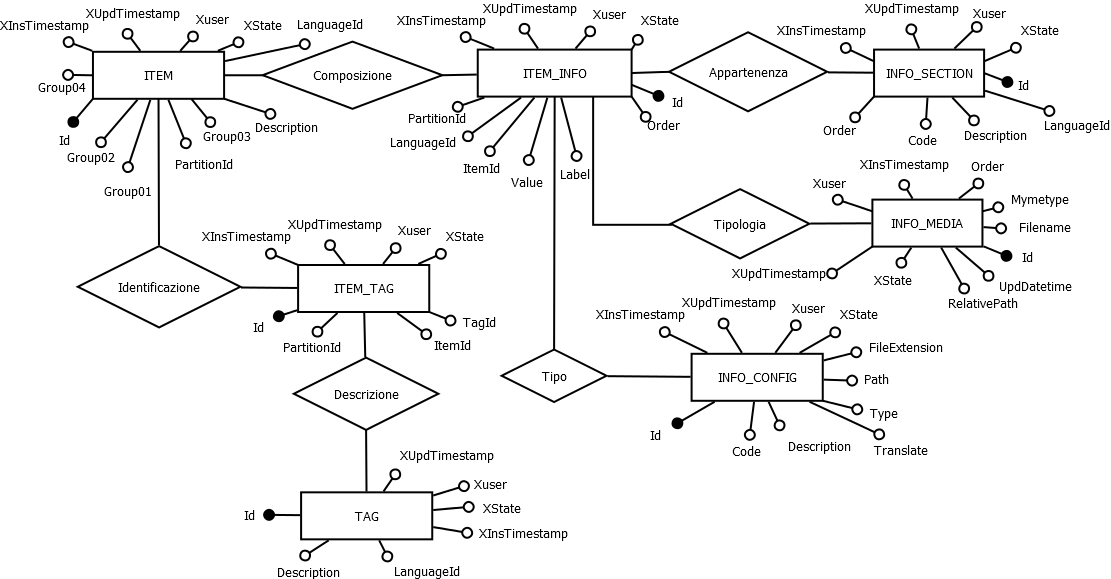
\includegraphics[width=1\columnwidth]{DiagrammaER} 
	\caption{Diagramma Entity Relationship}
	\label{DiagrammaER}
\end{figure}

Il diagramma ER (i vincoli sono fittizi, mostrano i collegamenti nonostante l'assenza di foreign key) è stato pensato in modo tale che ogni articolo disponga di molte informazioni appartenenti alle diverse categorie esistenti.

\paragraph{ITEM}
Questo oggetto è una vista contenente importanti informazioni. La fase di inserimento prevede unicamente che un'utente possa inserire alcune informazioni. I dati gestiti nella vista sono rappresentati dai gruppi di appartenenza (ad esempio insaccati, surgelati, prodotti da forno) ed una descrizione breve dell'oggetto.
In questo contesto la descrizione appare due volte: una negli ITEM ed una nella ITEM\_INFO per il semplice motivo che la tabella esisteva già nel database.

\paragraph{ITEM\_INFO}
La seguente tabella raggruppa tutte le informazioni e rappresenta il punto di collegamento dell'intero progetto. In essa vengono inserite le etichette e i valori che rappresentano i punti fondamentali di questa tabella. Le etichette (label) sono la descrizione dei valori (value) che permettono ricerche in tabella più rapide (video, titolo, immagine). I valori sono quelli che in base alle altre tabelle saranno stampati a video dall'applicazione web di front-end (\hyperref[ImgFrontend]{figura \ref{ImgFrontend}}).

\paragraph{INFO\_CONFIG}
La tabella INFO\_CONFIG è stata realizzata al fine di inserire dati in grado di limitare i tipi di record che possono essere gestiti all'interno della tabella ITEM\_INFO. Le informazioni raccolte permettono di gestire i record della tabella associata. Un esempio è dato dalla possibilità di definire le estensioni dei file.

\paragraph{INFO\_MEDIA}
INFO\_MEDIA è la tabella, come è comprensibile dal nome, che contiene tutte le informazioni relative ai file. Inizialmente, ho pensato di salvare il file nel database con un blob, in un secondo tempo ho convenuto che l'interrogazione di una tabella contenente molti media poteva diventare molto lenta considerando la richiesta di gestione dei video. Alla luce di queste riflessioni ho ritenuto opportuno ideare una cartella online in cui è installata l'applicazione, assegnare un GUID (nome univoco) al file e inserire nel database il percorso relativo dell'immagine.

\paragraph{INFO\_SECTION}
Le informazioni relative ad un prodotto devono essere categorizzate. INFO\_SECTION è una tabella che ha la funzione di indicare la categoria di appartenenza, così come, avviene in diversi siti e-commerce. L'obbiettivo è quello di gestire le informazioni presentandole in sezioni dinamiche. 

\paragraph{TAG}
TAG è una tabella che serve ad includere ogni tipo di parole chiave permettendo così di effettuare ricerche su prodotti o gruppo di prodotti. Questa tabella è stata riutilizzata perché già presente nel database.

\paragraph{ITEM\_TAG}
Quest'ultima tabella ha lo scopo di collegare i tag con il relativo articolo. Si è di fronte ad una relazione uno a molti che, in fase di ristrutturazione, ha comportato la creazione di una tabella intermedia tra articoli e tag.



\subsection{Design Pattern}
Durante la realizzazione dell'applicazione, si è notato che, per la maggior parte delle videate, un singolo oggetto doveva occuparsi di gestire le operazioni CRUD interne alla propria videata. Solo un caso particolare ha richiesto l'uso di un design pattern: la gestione di dettaglio del singolo articolo.
Il pattern scelto è il Facade. Tutte le informazioni partono da un articolo (record della tabella ITEM) e da questo vengono generate opportune operazioni.\\

\begin{figure}[!h] 
	\centering 
	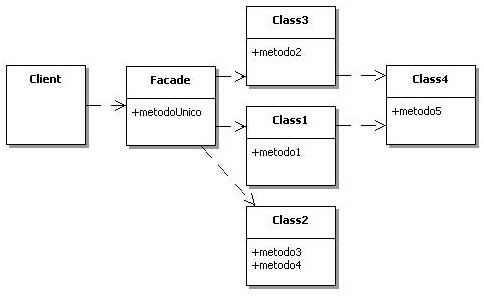
\includegraphics[width=1\columnwidth]{Pattern} 
	\caption{Design pattern strutturale: Facade (\url{https://bit.ly/2McTHsR})}
	\label{Pattern}
\end{figure}


Il grafico UML, generato una volta definito il design pattern da applicare, è risultato essere quello sottostante. Per realizzarlo, ho seguito la logica dell'applicazione e ho provato a sviluppare le attività di caricamento, creazione, modifica e cancellazione dei record delle diverse tabelle.

\begin{figure}[!h] 
	\centering 
	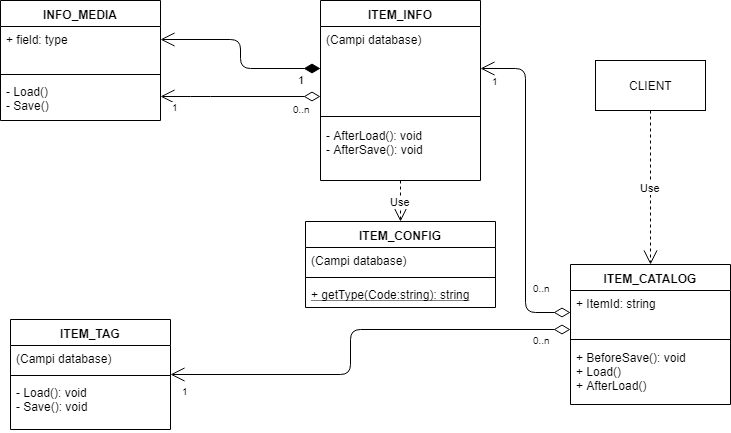
\includegraphics[width=0.7\columnwidth]{UML2} 
	\caption{Diagramma UML delle classi}
	\label{UML}
\end{figure}

%\subsubsection{Diagrammi di sequenza}
\paragraph{Caricamento}
Un dettaglio articolo non è altro che un'insieme di informazioni (ITEM\_INFO). Partendo da questo presupposto ho deciso di caricare un array di oggetti (in InDe prende il nome di IDCollection).
Per definire quale articolo carico, uso l'id dell'articolo; quindi eseguo la query. Quando ricevo una informazione verifico immediatamente a quale configurazione (INFO\_CONFIG) appartiene e solo se necessario carico gli ulteriori dati, ossia i media. Infine, con la classe ITEM\_TAG metto in un array tutti i tag associati all'articolo selezionato.

\paragraph{Creazione}
In questo caso, è necessario creare un articolo ITEM e poi prendere in esame gli ITEM\_INFO con o senza il proprio ITEM\_MEDIA. Poi, se vengono inseriti creo gli ITEM\_TAG. Tutto questo viene salvato unicamente dall'oggetto ITEM\_CATALOG permette di avviare gli eventi di save() dei vari oggetti.

\paragraph{Modifica}
In questo caso la modifica è uguale all'inserimento. La differenza è che nella fase di modifica dopo aver selezionato l'articolo desiderato, è caricata la videata di dettaglio con le informazioni che sarà possibile modificare a volte forzando l'update.

\paragraph{Cancellazione}
Ultima ma non meno importante è l' operazione di cancellazione. L'eliminazione di ogni singolo record di uno specifico articolo deve avvenire senza lasciare record orfani, pertanto la cancellazione ha inizio dai figli. L'ultima operazione manda in eliminazione l'articolo (ITEM) per il quale è prevista la cancellazione logica: cambio lo XState di un campo del record da "I" (Insert) o "M"(Modified) a "D" (Deleted) ed aggiorno XUpdDatetime.\\


\todo diagrammi di sequenza per le 4 operazioni


\section{Codifica}
Dopo la fase di progettazione, è stata affrontata la codifica. Questa fase è stata differente rispetto a quanto ho sviluppato durante il corso di Programmazione ad oggetti, Programmazione concorrente e distribuita ed Ingegneria del Software. La differenza o diversità è stata determinata dall'utilizzo di \inde.\\
Progettare classi e videate con questo tipo di software, ha cambiato il mio modo di implementare e testare. In precedenza il mio lavoro era organizzato in questo modo: creazione di una scaletta, implementazione e passo per passo effettuare dei test di unità basati su codice scritto (ad esempio Java associato a JUnit).\\
Diversamente in questo caso, ho saltato i test di unità, per passare immediatamente a test di sistema. Di conseguenza ho creato classi, metodi ed eventi cercando quanto più possibile di seguire una logica rigorosamente commentata. 
Rispetto alle mie aspettative di partenza, ho commesso un numero limitato di errori. Il codice generato si basa su template ben controllato e già testato dalla casa produttrice e con il debugger incluso, è stato possibile risolvere ogni errore commesso in tempi brevi  .


\subsection{Documenti}
\inde\ definisce con il termine documenti le classi java o c\# che dovranno essere generate e da cui si basano le applicazioni ideate.
Le prime classi che ho creato sono state quelle automatiche, secondo il ragionamento del framework ORM di InDe. Ho preso le tabelle del database e implementato una classe per ciascuna. Il funzionamento di alcune delle classi è rimasto quello standard. La classe che ha richiesto un  maggior ragionamento è stata quella per la gestione del dettaglio articoli.
La creazione automatica genera delle classi con tanti attributi quanti sono quelli presenti nelle tabelle di riferimento. Con essi sono creati anche i metodi get e set, rispettivamente dedicati a mostrare e modificare i valori di un record.

A seguito dell'utilizzo dell'ORM, le classi vengono generate sulla base di un template. Tutte le classi basate su un database estendono una classe IDDocument la quale contiene ogni metodo necessario ed evento necessario da gestire. Nelle classi derivate, create a partire da una tabella, è possibile intravedere nel codice come solo i metodi ed eventi di cui si hanno la necessità sono valorizzati e ridefiniti, mentre gli altri metodi previsti dal programma sono solo dichiarati e riprendono il funzionamento della classe padre.


%CONTINUARE CORREZIONE MARIA!!!!!

\subsubsection{ITEM}
La classe dedicata all'articolo è rimasta pressoché invariata. \'E stato creato inoltre un campo decodifica gruppi, al fine di mostrarlo a video e popolarlo solo in caso di esigenza. . Infine si è provveduto a rivedere la query da cui vengono estrapolati i dati da assegnare ad un oggetto.

\begin{center}
	\begin{tabular}{ p{3cm}|p{9,2cm} }
		\hline
		\textbf{Metodo e Query} & \textbf{Descrizione}\\
		\hline
		BeforeSave() & Questo metodo rientra tra quelli generati automaticamente dal programma. In aggiunta al normale funzionamento, ho inserito alcune informazioni da salvare in caso di inserimento, modifica o cancellazione (XState, XInsTimestamp, XUpdTimestamp). Nella cancellazione ho bloccato l'operazione di "delete" trasformandola in una "update" in cui il valore XState passa a "D".\\
		\hline
		DecodificaGruppi() & Il metodo di decodifica gruppi è stato realizzato al fine di caricare in un campo di tipo string l'insieme dei gruppi di appartenenza dell'Articolo, decodificando il codice nella descrizione corrispondente.\\
		\hline
		Master Query & Le master query sono le query di base che vengono lanciate per popolare gli attributi di una classe. In questo caso la modifica è finalizzata a limitare la visibilità ai soli record il cui campo XState non fosse "D", ovvero cancellato.\\
	
	\end{tabular}

\end{center}

\subsubsection{ITEM\_INFO}
Per quanto riguarda le informazioni, mi sono soffermato a lungo sul comportamento che l'oggetto dovrebbe avere dopo la lettura e il salvataggio dei dati nel database. 
\begin{center}
	\begin{tabular}{ p{3cm}|p{9,2cm} }
	%	\hline
	%	\multicolumn{2}{|c|}{ITEM\_INFO} \\
		\hline
		\textbf{Metodo e Query} & \textbf{Descrizione}\\
		\hline
		AfterSave() & Dopo aver salvato un oggetto di tipo ITEM\_INFO nel database, viene azionato questo metodo, utilizzato per controllare se l'informazione salvata è un'immagine. In tal  caso si procede all'inserimento di alcuni valori nell'oggetto Media.\\
		\hline
		AfterLoad() & Come per la AfterSave(), dopo aver caricato i record verifico di che tipo è. Se si tratta di un'immagine la carico nell'oggetto Media interno alla classe.\\
		
	\end{tabular}
\end{center}

\subsubsection{ITEM\_CONFIG}
La ITEM\_CONFIG è stata una delle prime classi a essere realizzata. Sulla base di questa sono gestiti alcuni eventi dell'ITEM\_INFO e dell'ITEM\_CATALOG. \'E stata studiata per contenere le configurazioni e ottenere in maniera rapida delle informazioni da altri oggetti. Per fare ciò ho creato metodi statici che effettuano query e restituiscono una specifica informazione.
\begin{center}
	\begin{tabular}{ p{4cm}|p{8,2cm} }
		%	\hline
		%	\multicolumn{2}{|c|}{ITEM\_INFO} \\
		\hline
		\textbf{Metodo e Query} & \textbf{Descrizione}\\
		\hline
		BeforeSave()		& Come per l'articolo anche in questo caso la cancellazione è stata gestita a livello logico.\\
		\hline
		GetFileExtension(string code)	& Metodo statico che restituisce un valore booleano in base al tipo di estensione se accettata o meno.\\
		\hline
		GetPath(string code) & Metodo statico che restituisce il percorso dove salvare i tipo (code) di file.\\
		\hline
		HasModal(string code) & Metodo che mi permette di controllare se questo tipo di ITEM\_CONFIG deve essere o meno gestito con l'uso delle modali.\\

	\end{tabular}
\end{center}

\subsubsection{INFO\_MEDIA}
La classe dedicata alla gestione dei media ha richiesto molto tempo rispetto al caricamento dei file nell'ITEM\_INFO. In fase di inserimento record nel database, è stato necessario ricercare un modo opportuno per salvare le immagini in una cartella dell'applicazione web con un nome univoco.
\begin{center}
	\begin{tabular}{ p{4,2cm}|p{8cm} }
		\hline
		\textbf{Metodo e Query} & \textbf{Descrizione}\\
		\hline
		OnEndTransaction() & Metodo che viene richiamato ogni qual volta si crea o modifica un singolo campo del database. Generalmente serve a popolare alcuni campi obbligatori ma non visibili. In questo caso è utilizzata per generare in automatico un path assoluto per permettere il caricamento dell'immagine. \\
		\hline
		BeforeSave()	& Prima di salvare il record, verifico se esiste già il file nella directory di destinazione. Se sì, confronto l'immagine precedente con quella appena caricata e solo se necessario salvo. Questo passaggio riduce il carico dei byte da trasferire.\\
		\hline
		AfterLoad()	& Carico il percorso assoluto dell'immagine e verifico se è presente una immagine in quel percorso. La assegno ad una variabile che a video verrà immediatamente esposta.\\
		\hline
		GetMediaPath()& Metodo che consente di ottenere il path dell'immagine.\\
		\hline
		ValorizzaImagePath(string TempPath)	& Metodo dedicato a creare una immagine temporanea nella cartella temporanea del programma che appena viene chiuso vengono cancellati automaticamente.\\
	
	\end{tabular}
\end{center}

\subsubsection{INFO\_SECTION e TAG}
Le seguenti due classi hanno mantenuto la gestione automatica generata da InDe. Tuttavia, anticipando quanto richiesto in un secondo momento, esposto nella sezione \ref{altriInterveti}, la classe INFO\_SECTION ha subito un cambiamento. Il cambiamento in questione è relativo alla gestione della lingua.

\subsubsection{ITEM\_TAG}
La classe è rimasta pressoché invariata da quella auto-generata nella gestione degli eventi fatta eccezione per l'inserimento e la modifica che ha richiesto solo l'arricchimento di dati di controllo.

\begin{center}
	\begin{tabular}{ p{5cm}|p{7,2cm} }
		%	\hline
		%	\multicolumn{2}{|c|}{ITEM\_INFO} \\
		\hline
		\textbf{Metodo e Query} & \textbf{Descrizione}\\
		\hline
		BeforeSave& Gestisco i campi XInsTimestamp, XUpdTimestamp e XState.\\
		\hline
		ExistsInCollection(IDCollection coll) & Metodo pubblico che individua se un elemento è presente nella IDCollection.\\
		
	\end{tabular}
\end{center}

\subsubsection{ITEM\_CATALOG}
Questa classe funge da tramite per tutte le operazioni relative al dettaglio di un prodotto. Essa non è basata su alcuna tabella. Nel caricamento delle informazioni vi sono specifiche query ideate per caricare unicamente la combinazione dei dati di un articolo. Si compone di due IDCollection una di ITEM\_INFO e una di ITEM\_TAG. La prima viene utilizzata per salvare le informazioni che vengono trasmesse, mentre la seconda viene utilizzata per salvare i tag.

\begin{center}
	\begin{tabular}{ p{3cm}|p{9,2cm} }
		%	\hline
		%	\multicolumn{2}{|c|}{ITEM\_INFO} \\
		\hline
		\textbf{Metodo e Query} & \textbf{Descrizione}\\
		\hline
		BeforeSave()& Questo evento rachhiude in sè il codice relativo all'inserimento, modifica e cancellazione dei dettagli articolo. Esso acquisisce le informazioni per mezzo dalle interfacce e richiama il salvataggio dei singoli ITEM\_INFO ed ITEM\_TAG, indicandone eventuali logiche a supporto.\\
		BeforeLoad()& L'oggetto non si basa su una tabella o una query. Esso fa riferimento a due collezioni di oggetti. Per caricare le due collezioni ho inserito dei campi obbligatori: ItemId, per riconoscere l'articolo, combinato al partitionId.  \\
		
	\end{tabular}
\end{center}


\subsection{Videate}
La creazione delle interfacce utente, chiamate anche "Videate" su Instant Developer, ha richiesto un lavoro di "drug and drop". Realizzare l' aspetto grafico è stato molto semplice e rapido, mentre l'aspetto "responsive" che ha richiesto una combinazione tra le funzionalità di InDe e l'importazione di un foglio di stile (Cascading Style Sheet) customizzato.
I metodi gestiti nelle videate riguardano gli eventi di load, refresh, update (che comprende inserimento, modifica e cancellazione dei record).\\

Tra tutte le videate realizzate, quelle più complesse sono state le interfacce dedicate al caricamento immagini. La loro realizzazione ha richiesto la gestione di alcuni comportamenti a livello di applicazione generale.
La gestione del file ha comportato continue revisioni. Il programma prevede che questi vengano caricati in una cartella temporanea. Tuttavia, in base a quanto definito in fase progettazione, una immagine viene salvata in una cartella ad essa dedicata con un nome univoco nella quale sono contenuti anche gli altri tipi di file. 
Prima di arrivare ad una soluzione definitiva, ho dovuto realizzare dei progetti di test. Da ultimo ho combinato insieme alcuni metodi dell'applicazione. In particolare ho unito il tempPath, metodo che restituisce il una stringa con il percorso alla cartella temporanea e il replace, metodo utilizzato per il rimpiazzo di stringhe. Infine, con un makeDirectory, altro metodo di InDe, ho creato il nuovo percorso dove salvare i file. 
L'insieme di questi metodi ha permesso di creare un nuovo percorso di salvataggio dei file. Per caricarli effettivamente ho optato per una doppia gestione: trascinamento dell'immagine nell'applicazione oppure click nella sezione di drop-down e importazione standard di documenti dal computer alla pagina web. 
Infine, per il caricamento ho optato per l'utilizzo della cache in modo tale da caricare i media di un elemento una sola volta per l'intera durata della sessione.\\

L'ultimo aspetto di focale importanza nella fase di codifica, è il controllo degli eventi onCommand() e load(). Il primo è lanciato ogni qual volta si prema un pulsante presente nell'intestazione della videata (refresh, save, insert, duplicate).  Il secondo è dedicato al caricamento delle videate ed a eventuali controlli prima di aprire una qualsiasi schermata.
Rispetto a quanto ambivo, la gestione del onCommand(), è risultata diversa per ogni videata.  Tuttavia, ho cercato di standardizzare il comportamento generale dell'applicazione seguendo i seguenti principi:
\begin{itemize}
	\item da una lista posso inserire, modificare e cancellare solo le principali informazioni;
	\item da una lista posso entrare nel dettaglio di un singolo elemento;
	\item dal dettaglio posso inserire dati, modificarli e cancellarli;
	\item dal dettaglio posso caricare media o dati particolari solo attraverso modali controllate (ad esempio nelle mail viene controllato che ci siano parole separate dal simbolo di \@ e da un punto).
\end{itemize}


\subsubsection{Modali}
Le modali sono videate di dimensioni ridotte, paragonabili ai popup, nelle quali ho dovuto gestire il caricamento di diverse informazioni. Per evitare di adottare una classe, anche per le modali ho adottato le tabelle IMDB. 
Una tabella IMDB è una sorta di "contenitore" temporaneo che mantiene le sue informazioni fino al termine della sessione. Le tabelle possono presentare uno o più record, i quali fungono da filtro all'apertura di una videata. Un esempio di suo utilizzo è stato l'inserimento delle variabili ItemId e PartitionId per filtrare un particolare articolo ed entrare quindi nel dettaglio di un singolo elemento.
Queste schermate sono state ideate al fine di passare dati alle videate sottostanti e si cancellano, alla chiusura, per non occupare memoria nella cache.


\section{Verifica, validazione e collaudo}
Le operazioni di verifica , validazione e collaudo sono risultate più semplici di quanto mi aspettassi. Per verificare il prodotto ho compilato il codice ed eseguito ogni volta l'applicazione. 
Appena eseguito il programma, ho seguito una scaletta pre-impostata con tutte le operazioni implementate e possibili. All'inizio ho commesso l'errore di creare molte funzionalità e poi testarle. Dopo 3 settimane ho concluso che è molto più vantaggioso concentrarsi su una singola funzionalità, farla funzionare correttamente e poi passare alla successiva.
Alla fine di ogni schermata, ho effettuato dei test generali sulle funzionalità e dopo un collaudo da parte del mio tutor, la videata  si considerava validata salvo eventuali errori.  
Il collaudo finale è stato gestito in maniera completamente diversa. Mentre la verifica e validazione sono state interne all'azienda e seguivano le linee guida indicate dai documenti di progetto, il collaudo è stato un rilascio anticipato al cliente. Quest'ultimo ha rieseguito i test da noi effettuati e ci ha rilasciato una lista delle nuove specifiche, miglioramenti o bug da risolvere. 
In seguito al fatto che, l'azienda segue la metodologia agile, i collaudi da parte del cliente sono stati più di uno. Grazie alla collaborazione tra fornitore e cliente, il progetto è stato portato a termine in maniera ottimale, permettendo di esplorare dei possibili miglioramenti.
Questi ultimi verranno esposti e illustrati nella sezione a seguire.

\section{Modulo RTC}
Il modulo RTC è un aspetto del progetto che non ho potuto approfondire a sufficienza. Nonostante ciò, ho potuto verificare che gli ideatori di \inde\ hanno previsto che ci potesse essere l'esigenza di creare una applicazione in lingua.
Il modulo RTC è un componente a pagamento utilizzabile solo con le licenze che lo includono. In questo modulo ci sono tre modalità di generazione delle traduzioni: google API key, Microsoft App Key e inserimento manuale. 
I primi due metodi di traduzione sono a pagamento, mentre la terza è sicuramente più economica ma richiede la conoscenza delle lingue in cui tradurre e il tempo per inserire le traduzioni.
La componente è semplice da integrare e, se si desidera, si può acquistare anche la sorgente ed apportare le modifiche desiderate al codice.
Lo studio effettuato ha avuto l'obiettivo di inserire il modulo in una fork del progetto.
 
\section{Altri interventi}\label{altriInterveti}
Il progetto ha subito un miglioramento ben evidente riguardante la gestione della lingua. L'applicazione web ideata deve poter creare informazioni sugli  articoli. In aggiunta, i dati inseriti devono apparire in pagine web di altre nazionalità. Per queste ragioni, mi è stato chiesto di tradurre o creare un metodo di inserimento delle stesse informazioni in qualsiasi altra lingua.

Per gestire la lingua, visto che la richiesta è nata in un secondo momento, ho deciso di inserire nelle tabelle un nuovo campo LanguageId popolato con l'identificativo della lingua individuabile in una tabella del database.
Introducendo questo nuovo campo, le classi lo hanno ereditato ed a questo punto ho cercato di studiare un modo per gestire le traduzioni. La soluzione è stata quella di introdurre un campo booleano nella tabella INFO\_CONFIG e un metodo statico isTranslatable(string code), i quali mi indicavano se un campo deve essere tradotto oppure no, come nel caso delle immagini.
Per lasciare completa libertà all'utente ho deciso di inserire il campo a video nella videata dedicata alle configurazioni in modo tale che, se un utente vuole anche che le immagini cambino in seguito alla lingua è possibile farlo attraverso una check-box.

Le classi modificate a seguito del campo LanguageId sono state ITEM, ITEM\_INFO, INFO\_SECTION, INFO\_CONFIG. Le modifiche hanno influito su tutti i caricamenti e i salvataggi. Nel primo caso si è aggiunta alla clausola where delle master query il languageId, mentre nel secondo si è inserito un controllo della lingua.
